\documentclass[output=paper]{LSP/langsci}
\author{Gianluca Pontrandolfo}
\title{Investigating judicial phraseology with COSPE: A contrastive corpus-based study}
%\epigram{Change epigram in chapters/01.tex or remove it there }
\abstract{This chapter describes the results of an empirical study of \textsc{lsp} phraseological units in a specific domain (criminal law) and type of legal genre (criminal judgments). The final goal of the research is to provide legal translators with a multifunctional resource having a positive impact on the translation process and product. More specifically, it aims at assisting translators – as well as legal experts – to develop their phraseological competence through \todo{I deleted a `their' here to fit the line} exposure to real, authentic (con)texts in which these phraseological units are used. Based on \textsc{cospe}, a 6-million trilingual, comparable corpus of criminal judgments, this study approaches phraseology from a contrastive (Spanish-Italian-English), quantitative and qualitative perspective. Corpus analysis and term extraction have been carried out by means of concordancers (mainly WordSmith Tools v. 5.0).
From a methodological point of view, the study combines corpus-based and corpus-driven approaches, as well as traditional approaches applied to Language for General Purposes (LGP) phraseology, and more recent distributional studies of Language for Specific Purposes (LSP) and legal phraseology. Emphasis is placed on four categories of phraseological units frequently found in judicial discourse: complex prepositions, lexical doublets and triplets, lexical collocations and routine formulae.}
\maketitle
\rohead{\thechapter\hspace{0.5em}Investigating judicial phraseology with \textsc{cospe}} % Display short title
\begin{document}
\section{Introduction}
 Legal translation is not only a question of terminology – which is indeed one of the major obstacles legal translators have to face in their daily activity – but also a question of phraseological conventions. Beyond lexical and terminological equivalence, translators have to tackle the additional difficulty of acquiring familiarity with the genre structures – or “generic” structures in \citeauthor{Hasan1978}'s (\citeyear{Hasan1978}) terms – through which legal institutions conduct their affairs. \citet[190]{Hatim1990} use the term “routines” to describe “those conventions which translators either know or simply do not know: frozen patterns of a formulaic nature which are typical of legal texts and which can be translated only resorting to parallel routines in the target language”. As a matter of fact, even the most skilled translator may run the risk of producing a translation that is inaccurate from the standpoint of the “register choices”, all other aspects of the target text being perfectly acceptable (grammar, content, etc.) \citep[see][218--219]{Garzone2007}.
 
The current studies of phraseology in specialised registers acknowledge the need for corpus-based studies of the prototypical lexico-grammatical patternings and discourse functions of lexical phrases across disciplines. Gaining control of a new language or register requires, following \citet[5]{Hyland2008}, a sensitivity to expert users’ preferences for certain sequences of words over others that might seem equally possible.
 
In line with these preliminary remarks, the study stems from three main considerations:

\begin{enumerate}
\item Judgments represent a fertile ground for the study of phraseology: the frequent use of phraseological units is one of the most striking features of these judicial texts, a real “trademark” of legal texts \citep[154]{Mortara2001};
\item Phraseology is one of the main obstacles legal translators have to tackle in their professional activity \citep[see][]{Garzone2007,Kjaer2007};
\item Confronted with the task of translating legal texts, professional translators have few phraseological resources at their disposal.
\end{enumerate}

The relation between “phraseology”, “judicial texts” and “translation” appears to have been scarcely investigated so far. The research has represented a first, tentative step towards filling such gap.\footnote{This chapter is based on a PhD research project conducted on specialised phraseologies employed in criminal judgments \citep{Pontrandolfo2013a}. The PhD thesis entitled “La fraseología en las sentencias penales: un estudio contrastivo español, italiano, ingles basado en corpus” (Supervisor: Helena Lozano Miralles; Co-supervisors: Emilio Ortega Arjonilla, Mitja Gialuz) was defended by the author on 12/04/2013 at the University of Trieste within the XXV PhD cycle in Interpreting and Translation Studies (coordinator: Federica Scarpa). The contribution is also based on a conference paper given during the 19th European Symposium on Languages for Special Purposes, 8--10 July 2013 held at the University of Vienna. It is part of the research project titled “Elaboración de una subontología terminológica (español, inglés e italiano) a partir de FunGramKb: cooperación internacional en materia penal (terrorismo y crimen organizado)”, whose lead researcher is Ángel Miguel Felices Lago (University of Granada), funded by the Spanish Ministry of Science and Innovation (code: FFI2010-15983/FILO).}

\section{Theoretical background}
Phraseology in legal and judicial language is a rather unexplored field of study. The following literature survey of the relevant sources, concepts and definitions is structured into three main parts:

\begin{enumerate}
\item Phraseology. A number of influential classifications of phraseological units have been analysed in \textsc{lgp} (from the seminal work of \citealt{Benson1986,Corpas1996,Gläser1994/1995,Glaeser1998,Ruiz1997,Cowie1988,Cowie2001,Melchuk1998, Moon1998,Burger1998,Granger2008}), \textsc{lsp}  \citep{Homme2000,Lorente2001,Tercedor1999,Montero2002,Bevilacqua2004,Aguado2007} and legal phraseology \citep {Kjær1990,Kjaer1990b};
\item Corpora for the study of legal and judicial language \citep[see][]{Pontrandolfo2012}. After presenting the main definitions and concepts, the review focuses on the main corpora built in Spain (e.g. \textsc{jud}-\textsc{gentt}, the \textsc{iula}’s \textsc{corpus}, \textsc{cluvi}), Italy (e.g. BoLC, \textsc{coris}/\textsc{codis}, \textsc{cadis}), England and Wales (e.g. Cambridge Corpus of Legal English, HOLJ Corpus, Proceedings of the Old Bailey), as well as in the European Union and the rest of the world;
\item Studies carried out by researchers from different areas and schools dealing with the topic of the present research, as the subject or a side aspect of their investigations.
\end{enumerate}

As far as the third part is concerned, research in this area can be classified into four different subareas, according to the methodological approach, the types of phraseological units investigated as well as the focus of the analysis:

\begin{enumerate}
\item[a)] Studies that analyse lexico-syntactic combinations in legal language, with a preference for specialized collocations, based on the traditional notion of phraseology \citep{Benson1986,Hausmann1989,Corpas1996,Berdychowska1999, Nardon2002,Lombardi2004,Rovere1999,Nystedt2000,Cruz2002,Giráldez2007,
Anderson2006,Montenegro2007,Biel2011,Bhatia2004};      
\item[b)] Studies that focus on the formulaic nature of legal language in terms of routine formulae \citep{Rega2000,Bachmann2000,Monzo2001,Carvalho2007,Giurizzato2008};
\item[c)] Lexicographic studies aimed at building specialised legal dictionaries \citep{Groot1999,François1997,Gisbert2008,Fernández2008};
\item[d)] Studies that adopt a wider notion of phraseology and are based on large corpora of legal texts aimed at analysing co-occurrence patterns \citep{Mazzi2005,Mazzi2010,GozdzRoszkowski2011}.
\end{enumerate}

The survey highlighted a significant gap in the literature on translation-orient\-ed studies of the phraseological nature of legal or judicial discourse, as there are still only few studies dealing with the role of phraseology in judicial discourse from an empirical, contrastive, corpus-based perspective. 

\section{Aim, scope and objectives of the research}
The study deals with the complex universe of phraseology, in its broader sense \citep[see][6]{Gries2008}, from a contrastive (Spanish--Italian--English), quantitative and qualitative perspective. Emphasis has been placed on a specific genre, criminal judgments, i.e. “courts’ final determination of the rights and obligations of the parties in a case” \citep[see][918]{Bryan2009}.

Judgments epitomise the nature of judicial discourse, as they are the most important acts in criminal trials, and represent one of the most striking examples of “living law” or “law in action” to refer to the 1910’s pioneer paper by the distinguished legal scholar Roscoe Pound (see \citealt[154]{Garavelli2010}; \citealt[253]{Cadoppi1999}). Studying judgments means exploring the language of the discourse community composed by judges. Narrowing down the huge normative subjects the courts are asked to rule on has allowed to focus on a coherent and consistent share of case-law. Furthermore, this has left room for a long-term study that could delve into the correlation between a specific field of law (e.g. civil, labour law, etc.) and the type of phraseological patterns used by legal experts.

The research questions lying at the basis of the study can be summarised as follows:

\begin{enumerate}
\item Phraseology is a key stylistic feature of criminal judgments, a real “trademark” in judges’ writing conventions. \textit{What is the quantitative and qualitative relevance of this typological trait in criminal judgments}? 
\item Due to the different legal traditions (common law vs. civil law) characterising the three cultures involved in the present study (Spain, Italy, and England and Wales), \textit{does the weight of phraseological units change depending on the respective source country}? 
\item Once a selected number of phraseologisms have been extracted, \textit{will it be possible to establish a comparability between them}?
\end{enumerate}

The main goal of this empirical study of specialised phraseological units in a specific type of legal genre, i.e. criminal judgments, is that of providing legal translators dealing with criminal procedure with a multifunctional resource having a positive impact on the translation process and product. More specifically, it aims at assisting legal translators (as well as legal experts) in developing phraseological competence, guiding them to achieve “naturalness” in writing through exposure to real, authentic (con)texts in which phraseological units are used.

\section{Material}
In order to answer the research questions, a trilingual, comparable corpus of judicial texts has been built, i.e. the Corpus of Criminal Judgments (\textit{COrpus de Sentencias PEnales}, \textsc{cospe}). The focus has been placed on a single genre (criminal judgments) for a number of reasons \citep[see][171--181]{Pontrandolfo2013a}. Among them, the importance of this specific genre in judicial discourse – see the importance of the judicial “precedent” in the common-law as well as civil-law traditions – and, from a practical point of view, the need to find a shared ground across legal cultures to allow for a full comparative analysis.

As \citet[156--157]{Hunston2008} put it, “all corpora are a compromise between what is desirable, that is, what the corpus designer has planned, and what is possible”. Tab. 1 shows the result of a number of strategic decisions which have been taken and challenges which have been tackled to compile a balanced legal corpus. As shown in Tab. 1, \textsc{cospe} is made of two subcorpora: \textsc{cospe}-\textsc{S}up which gathers 380 criminal judgments delivered between 2005 and 2012 by the Supreme Courts (courts of last instance) in the three judicial systems, and \textsc{cospe}-\textsc{A}p which contains 402 criminal judgments delivered in the same period by various courts of appeal (courts of second instance) in Spain, Italy, and England and Wales. These courts have been chosen for being comparable in terms of role and functions.


\begin{table}
     \centering
     \begin{tabular}{llrr}
     \lsptoprule
%\textbf{\textsc{cospe}} (Corpus of Criminal Judgments)&&& \\
Type of corpus: & Trilingual, comparable && \\
Languages: & ES-IT-EN && \\
Size: & Tot. \textbf{782} txt (\textbf{6,036,915} tokens) && \\
Genre: & Criminal Judgments && \\
Period: & 2005 - 2012 && \\
Purposes: & Pratice, Research, Training   && \\
     \lsptoprule
       \textbf{ES}  & \textbf{Court}       & \textbf{txt}  &  \textbf{tokens} \\ \midrule
       \textbf{\textsc{cospe}-\textsc{S}up}    & \textit{Tribunal Supremo}          & 100				& 1,088,770\\
       \textbf{\textsc{cospe}-\textsc{A}p}       & \textit{Audiencia Provincial}    & 127				& 722,177\\
                     & \textit{Tribunal Superior de Justicia}      & 35				& 208,619\\
                      & tot             & 162				& 930,796\\ \midrule
       \textbf{\textsc{cospe}-ES (tot.)}    &              & \textbf{262}				& \textbf{2,019,566}\\ 

\lspbottomrule
       \textbf{IT}  & \textbf{Court}       & \textbf{txt}  & \textbf{tokens} \\ \midrule
       \textbf{\textsc{cospe}-\textsc{S}up}    & \textit{Corte Suprema di Cassazione}             & 230				& 1,014,224\\
       \textbf{\textsc{cospe}-\textsc{A}p}       & \textit{Corte d’Appello}             & 95				& 357,057\\
                     & \textit{Corte d’Assise d’Appello}             & 40				& 629,905\\
                      & tot             & 135				& 968,962\\ \hline
       \textbf{\textsc{cospe}-IT(tot.)}   &    &     \textbf{365}				& \textbf{2,001,186}\\  
\lspbottomrule

       \textbf{EN}  & \textbf{Court}       & \textbf{txt}  & \textbf{tokens} \\ \midrule
       \textbf{\textsc{cospe}-\textsc{S}up}    & \textit{Supreme Court}             & 20				& 428,529\\
       \textbf{\textsc{cospe}-\textsc{S}up}       & \textit{House of Lords}         & 30				& 455,468\\
                                & tot     & 50				& 883,997\\
       \textbf{\textsc{cospe}-\textsc{A}p}  & \textit{Court of Appeal} & 105				& 1,132,166\\ \midrule
       \textbf{\textsc{cospe}-EN(tot.)}   &    &     \textbf{155}				& \textbf{2,016,163}\\  
\lspbottomrule
\end{tabular}
 
\caption{Composition of \textsc{cospe} (Corpus of Criminal Judgments)}
     \label{tab:6.3}
     % Verweis im Text mittels \REF{tbl:beispieltabelle}
\end{table} 

With a view to obtaining a representative sample of the genre \citep[see][243]{Biber1993}, a number of variables have been established to guarantee heterogeneity and balance in the process of storing and categorising the judgments, as well as to ease its consultation and queries: ID number, division of the court, region/city (to guard against diatopic usage), date of the hearing, subject matter (to vary the relationship between phraseology and specialised contents), type of proceedings, reporting judge (to guard against idiosyncratic usage), notes (e.g. outcome of the appeal, final decision of the court, etc.).

Following \citet[105--107]{Zanettin2012}, \textsc{cospe} is a “translation-driven corpus” in that it has been created with applied (translation) purposes in mind and it does not include translated texts, but texts produced in the three languages under similar circumstances and within the same domain. It is also a “web corpus” (“corpus virtual” according to Corpas Pastor 2004: 227) in that all the texts have been collected from the web (from \textsc{cendoj}, DeJure, Bailii databases) and were therefore already available in electronic format. \textsc{cospe} is currently being \textsc{pos}-tagged.

The corpus has represented the test bed for the investigation based on the research questions which have been tackled adopting a corpus-based methodology.

\section{Methodology}
The study is a descriptive, empirical research which has fully adopted the corpus linguistics paradigm \citep[see][]{McEnery2006}. Phraseology in criminal judgments has therefore been approached through “real judicial life” examples. Extraction and analysis of relevant phraseologisms have been performed by means of concordancers (mainly WordSmith Tools, but also AntConc and ConcGram).

Querying a corpus of large dimensions like \textsc{cospe} inevitably requires the adoption and integration of different methods, according to the different types of phraseological unit. Methodologies for phraseology extraction vary along a continuum having the manual analysis on one side and the automatic one on the other. Such dichotomy is also reflected in the corpus-driven vs. corpus-based approaches to phraseology, or, to put it in \citeauthor{Granger2005}'s (\citeyear{Granger2005}:3) terms, between the \textit{bottom-up approach}/corpus-driven (an inductive approach generates a wide range of word combinations, which do not all fit predefined linguistic categories) and the \textit{top-down approach}/corpus-based (which identifies phraseological units on the basis of linguistic criteria).

Tab. 2 shows the methodological moves adopted to extract the phraseological units around the four types object of the investigation, along the continuum corpus-based vs. corpus-driven.

\begin{table}
     \centering
     \resizebox{\textwidth}{!}{
     \begin{tabular}{llll}
     \lsptoprule
       \textbf{+ corpus-based}  &        &   & \textbf{+ corpus-driven} \\ \midrule
       \textbf{Complex prepositions}    & \textbf{Lexical doublets/triplets}             & \textbf{Lexical collocations}	& \textbf{Routine/Standardised formulae}\\
       Semi-manual extraction       & Semi-automatic extraction        & Semi-automatic extraction				& Automatic extraction \\
       (e.g. in + * + with)             & (e.g. * + and + *)     & (MI score\footnote{“A measure of how strongly two words seem to associate in a corpus, based on the independent relative frequency of two words” \citep{Church1990}.} of a selection of nodes/key terms\footnote{To identify the nodes of the collocations an innovative method has been followed based on Schank and Abelson’s notion of “script” – “a structure that describes appropriate sequences of events in a particular context” \citet[141]{Schank1977} – adapted to the context of criminal judgments of second or last instance (e.g. During a \textit{trial} the \textit{Court/judge} issues a \textit{judgment} against a person accused of a crime, i.e. a \textit{defendant} who committed an \textit{offence}. The \textit{appellant} contests the court’s decision adducing his/her \textit{arguments}. The Court can allow or dismiss the appeal (acquitting or convicting him/her), (re)determining the \textit{sentence}. The judge explains his/her \textit{opinion}]. Starting from the script, nine key terms have been identified – ES: \textit{juicio, tribunal/juez, acusado, delito, sentencia, motivo, recurso, apelante/recurrente, pena}; IT: \textit{giudizio, giudice/corte/tribunale, imputato, reato/delitto, sentenza, motivo, ricorso/appello, appellante/ricorrente, pena}; EN: \textit{trial, court/judge, defendant, offence, judgment/decision/opinion, argument, appeal, appellant, sentence} – and later scrutinised to discover phraseological patterns.})	& (WS ConcGram and ConcGram 1.0)\\  \midrule
       \textbf{top-down approach}      & 				&       & \textbf{bottom-up approach} \\ 
 \lspbottomrule      
\end{tabular}
 }
\caption{Methods of extraction along the continuum corpus-based vs. corpus-driven}
     \label{tab:6.4}
     % Verweis im Text mittels \REF{tbl:beispieltabelle}
\end{table}

To retain methodological rigour, a cut-off point of 5 occurrences per 2,000,000 words has been fixed, combined with the multiple-text requirement whereby a given phraseological unit had to appear in at least 5 different judgments to guard against judges’ idiosyncrasies \citep[110]{GozdzRoszkowski2011}.
The extraction has yielded a significant numbers of specialised phraseological units which will be dealt with in the following sections.

\section{Results}
A quantitative and qualitative analysis of the four types of recurrent phraseological units mentioned above has been carried out. The following sections contain a summary of the findings that, for reasons of space, cannot be presented exhaustively in this paper.
\subsection{Complex prepositions}
Following \citet[75]{Biber1999}, “complex prepositions are multi-word sequences that function semantically and syntactically as single preposition”, i.e. “grammaticalised combinations of two simple prepositions with an intervening noun, adverb or adjective” \citep[44]{Granger2008}. There can be two types of complex prepositions: N + P (e.g. ES: \textit{encima de}; IT: \textit{innanzi a}; EN: \textit{owing to}) and P + N + P (e.g. ES: \textit{con arreglo a}; IT: \textit{in ordine a}; EN: \textit{in accordance with}).

These phraseological units, especially the second type, are highly frequent in Spanish, Italian and English legal language \citep[see][]{Pontrandolfo2013b}, as can be seen from the examples taken from \textsc{cospe}:

\begin{itemize}
\item \textbf{ES}: \textit{al amparo de, a juicio de, en aras de, en concepto de, a instancia(s) de}, etc.
\item \textbf{IT}: \textit{in relazione a, in ordine a, a titolo di, in conformità a, in deroga a, a pena di}, etc.
\item \textbf{EN}: \textit{on behalf of, by reason of, without prejudice to, by virtue of, on the ground(s) of}, etc.
\end{itemize}

\figref{fig:6:1} shows the quantitative results in terms of total number, total number of patterns (e.g. as + * + as; by + * + of; etc.) vs. number of types (single different combinations such as “with reference to”, “without prejudice to”, etc.).

\begin{figure}
% 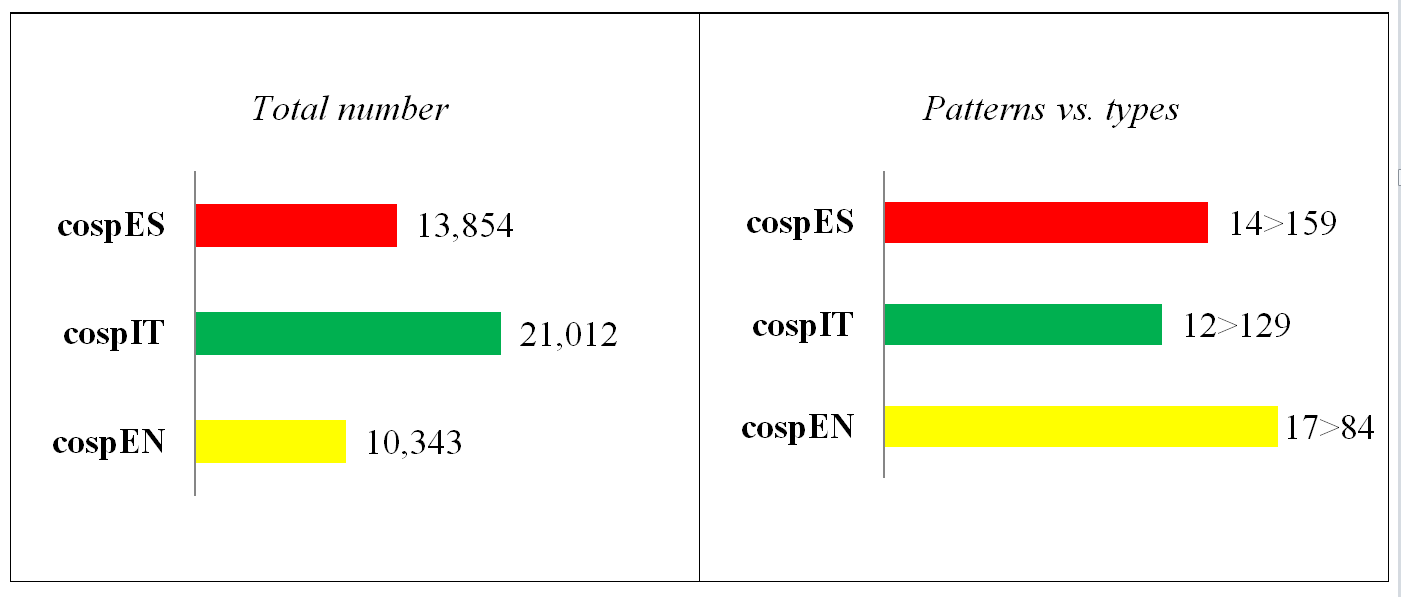
\includegraphics[width=1.0\textwidth]{./figures/1-1.png}
\definecolor{LSPdarkgreen}{RGB}{0,176,80}
\resizebox{\textwidth}{!}{
\begin{tikzpicture}[]
\begin{axis}[title=\emph{Total Number}, xbar, y=1cm, axis x line=none, axis y line*=left, nodes near coords, nodes near coords align=horizontal, xmin=5000, ytick={1,2,3}, yticklabels={cospEN,cospIT,cospES}, width=.4\textwidth, height={}, tickwidth=0pt, bar shift=0, bar width=10, enlarge y limits=0.2, every node near coord/.append style={yshift=-9pt, xshift=20pt}]
		
\addplot [draw=none, fill=yellow, point meta=explicit symbolic] coordinates {(10343,1) [10,343]};
\addplot [draw=none, fill=LSPdarkgreen, point meta=explicit symbolic] coordinates {(21012,2) [21,012]};
\addplot [draw=none, fill=red, point meta=explicit symbolic] coordinates {(13854,3) [13,854]};
		
\end{axis}
\end{tikzpicture}
\hspace{1cm}
\begin{tikzpicture}
\begin{axis}[title=\emph{Patterns vs. types}, xbar, y=1cm, axis x line=none, axis y line*=left, nodes near coords, nodes near coords align=horizontal, xmin=0, ytick={1,2,3}, yticklabels={cospEN,cospIT,cospES}, width=.4\textwidth, height={}, tickwidth=0pt, bar shift=0, bar width=10, enlarge y limits=0.2, every node near coord/.append style={yshift=-7pt, xshift=20pt}]
		
\addplot [draw=none, fill=yellow, point meta=explicit symbolic] coordinates {(17,1) [17\textgreater 84~]};
\addplot [draw=none, fill=LSPdarkgreen, point meta=explicit symbolic] coordinates {(12,2) [12\textgreater 129]};
\addplot [draw=none, fill=red, point meta=explicit symbolic] coordinates {(14,3) [14\textgreater 159]};
		
\end{axis}
\end{tikzpicture}
}
\caption{Complex prepositions (N + P + N) (quantitative findings)} \label{fig:6:1}
\end{figure}

The Spanish subcorpus (CospES) presents a wider variety of complex prepositions (159 different types generated by 14 patterns), compared with the Italian one (CospIT) (129 vs. 12) and the English one (CospEN) (84 vs. 17). This seems to suggest that, although the Italian judgments contain the highest number of complex prepositions (21,012), they tend to be much more repetitive than their Spanish and English counterparts. Indeed, the 21,012 complex prepositions are always made of the same patterns (12) which compose 129 different types. CospES displays a lower number of instances (13,854), although the types seem to generate a wider number of phraseological units (159). CospEN shows the lowest number of occurrences (10,343), even though the range of prepositional patterns is much wider (17), but less significant quantitatively (84 different types of complex prepositions stemming from 17 formal structures).

As far as the qualitative analysis of the results is concerned, obviously not all the complex prepositions detected are typical of judicial language. In order to uncover those phraseological units which are used with a certain preference by judges, a comparison between the relative frequency of these patterns in \textsc{cospe} and their frequency in reference corpora (\textit{\textsc{crea}} and \textit{Corpus del Español} for Spanish, \textit{\textsc{coris}/\textsc{codis}} for Italian, \textit{\textsc{bnc}} for English) has been conducted. “By virtue of”, for example, is used with a raw frequency of 26 in CospEN (normalised frequency of 12.90 per million words), whereas in the \textsc{bnc} it has a frequency of 19 (normalised frequency 0.19 per million words). It is therefore much more used in legal and judicial language. The same applies to “in furtherance of” which has no occurrences in the \textsc{bnc} (vs. 37 instances in 13 different texts in CospEN). The full list of complex prepositions used much more frequently in judicial language can be found in \citet[200--205]{Pontrandolfo2013b}.

\subsection{Lexical doublets and triplets}
Following \citet[90]{Bhatia1984}, “binomial or multinomial expressions are sequences of two or more words or phrases belonging to the same category having some semantic relationship and joined by some syntactic device such as \textit{and} or \textit{or}”. The following examples are all taken from \textsc{cospe}:

\begin{itemize}
\item \textbf{ES}: \textit{pronunciamos, mandamos y firmamos, [debo] absolver y absuelvo, real y efectivo, natural y vecino}, etc.
\item \textbf{IT}: \textit{illogica e contraddittoria, penale e processuale, rigetta e condanna, previsto e punito, connesso e collegato}, etc.
\item \textbf{EN}: \textit{adequate and proper, fair and public, reasoning and conclusions, stop and search}, etc.
\end{itemize}

\figref{fig:6:2} shows the quantitative results of the doublets extracted from \textsc{cospe} (triplets do not play a crucial role in the genre under investigations).

\begin{figure}
% 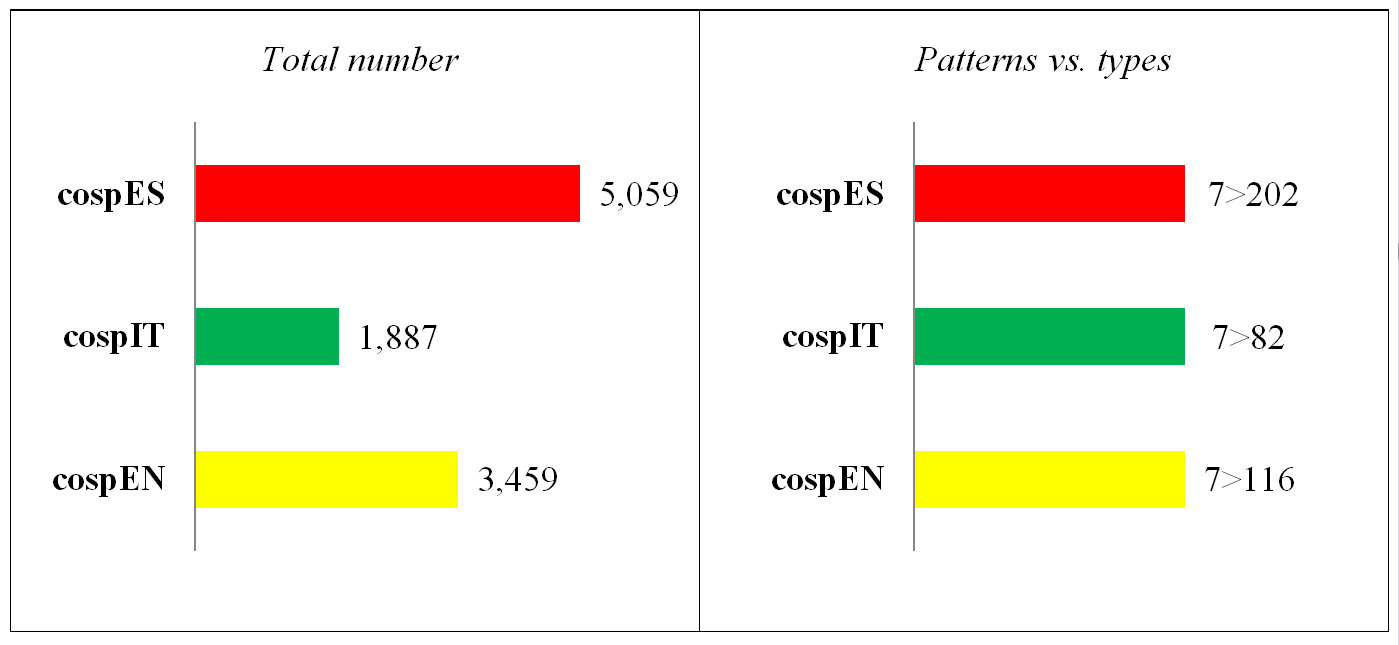
\includegraphics[width=1.0\textwidth]{./figures/1-2.png}
\definecolor{LSPdarkgreen}{RGB}{0,176,80}
\resizebox{\textwidth}{!}{
\begin{tikzpicture}[]
\begin{axis}[title=\emph{Total Number}, xbar, y=1cm, axis x line=none, axis y line*=left, nodes near coords, nodes near coords align=horizontal, xmin=1000, ytick={1,2,3}, yticklabels={cospEN,cospIT,cospES}, width=.4\textwidth, height={}, tickwidth=0pt, bar shift=0, bar width=10, enlarge x limits=0, enlarge y limits=0.2, every node near coord/.append style={yshift=-9pt, xshift=20pt}]
		
\addplot [draw=none, fill=yellow, point meta=explicit symbolic] coordinates {(3459,1) [3,459]};
\addplot [draw=none, fill=LSPdarkgreen, point meta=explicit symbolic] coordinates {(1887,2) [1,887]};
\addplot [draw=none, fill=red, point meta=explicit symbolic] coordinates {(5059,3) [5,059]};
		
\end{axis}
\end{tikzpicture}
\hspace{1cm}
\begin{tikzpicture}
\begin{axis}[title=\emph{Patterns vs. types}, xbar, y=1cm, axis x line=none, axis y line*=left, nodes near coords, nodes near coords align=horizontal, xmin=0, ytick={1,2,3}, yticklabels={cospEN,cospIT,cospES}, width=.4\textwidth, height={}, tickwidth=0pt, bar shift=0, bar width=10, enlarge x limits = 0, enlarge y limits=0.2, every node near coord/.append style={yshift=-7pt, xshift=20pt}]
		
\addplot [draw=none, fill=yellow, point meta=explicit symbolic] coordinates {(7,1) [7\textgreater 116]};
\addplot [draw=none, fill=LSPdarkgreen, point meta=explicit symbolic] coordinates {(7,2) [7\textgreater 82~]};
\addplot [draw=none, fill=red, point meta=explicit symbolic] coordinates {(7,3) [7\textgreater 202]};
		
\end{axis}
\end{tikzpicture}
}
\caption{Lexical doublets (quantitative findings)} \label{fig:6:2}
\end{figure}

The analysis showed a proportionality between the total number of instances and the types generated by the 7 patterns identified in the three subcorpora. CospES contains the highest number of types (202) and tokens (5,059), followed by CospEN (3,459 distributed over 116 types) and CospIT (1,887 vs. 82).

The quantitative analysis revealed that the most frequent doublets are those made of two nouns (45\% in CospES, 56\% in CospIT and 34\% in CospEN) – e.g. \textit{violencia e intimidación}, \textit{contraddittorietà e dillogicità}, \textit{the prosecution and the defence} – followed by the patterns made of two verbs (22\% in CospES, 9\% in CospIT and 11\% in CospEN) – e.g. \textit{previsto y penado}, \textit{rappresentato e difeso}, \textit{aiding and abetting}) – and those made of two adjectives (16\% in CospES, 16\% in CospIT and 25\% in CospEN), e.g. \textit{oral y público}, \textit{connesso e collegato}, \textit{noble and learned}. Lexical doublets made of prepositions (e.g. \textit{unless} and \textit{until}), articles, pronouns (e.g. \textit{he or she}) and adverbs (e.g. \textit{before and during}) seem to be used much more frequently in \textsc{lgp} rather than in legal language.

The comparison with the reference corpora confirms that lexical doublets are used much more frequently in judicial language. “Adequate and proper”, for example, is used with a raw frequency of 15 in CospEN (normalised frequency of 7.43 per million words), whereas in the \textsc{bnc} it has a frequency of 3 (normalised frequency 0.03 per million words).

\subsection{Lexical collocations}
Following \citet[43]{Granger2008}, “lexical collocations are usage-deter\-mined or preferred syntagmatic relations between two lexemes in a specific syntactic pattern. Both lexemes make an isolable semantic contribution to the word combination but they do not have the same status. Semantically autonomous, the base of a collocation is selected first by language user for its independent meaning. The second element, i.e. the collocate/collocator, is selected by and semantically dependent on the base”.

The analysis conducted on \textsc{cospe} has been based on nine key terms (see note \textit{b}) as base of the \enlargethispage{1\baselineskip} collocation. As a matter of fact, specialised terminology tends to cluster around terms. Phraseology acts as a link between the term and the text. In particular, the analysis has focused on four types of collocations, exemplified as follows:

\begin{enumerate}
\item\textbf{ N [subject] + V}
\begin{itemize}
\item \textbf{ES}: \textit{valorar una sentencia, carecer un motivo, celebrar un juicio, entender un tribunal}, etc.
\item \textbf{IT}: \textit{sussistere un reato, ritenere la corte, osservare il giudice}, etc.
\item \textbf{EN}: \textit{plead guilty/not guilty an appellant, hold the court, conclude the judge}, etc.
\end{itemize}
\item \textbf{V + N [object]}
\begin{itemize}
\item \textbf{ES}: \textit{esgrimir un motivo, aducir un motivo, cometer un delito, condenar al acusado}, etc.
\item \textbf{IT}: \textit{irrogare una pena, proporre un ricorso, accogliere un ricorso, adire la corte}, etc.
\item \textbf{EN}: \textit{to convict/acquit a defendant, to allow/dismiss an appeal, to await trial, to impose a sentence}, etc.
\end{itemize}
\item \textbf{N + \textsc{adj}}
\begin{itemize}
\item \textbf{ES}: \textit{motivo impugnatorio, motivo decisorio, pena accesoria}, etc.
\item \textbf{IT}: \textit{giudice a quo, imputato contumace, sentenza contraddittoria}, etc.
\item \textbf{EN}: \textit{appropriate sentence, reduced sentence, leading judgment, honest opinion}, etc.
\end{itemize}
\item \textbf{N + prep + N}
\begin{itemize}
\item \textbf{ES}: \textit{celebración del juicio, desestimación del recurso, anulación de la sentencia}, etc.
\item \textbf{IT}: \textit{rigetto del ricorso, entità della pena, accoglimento del motivo}, etc.
\item \textbf{EN}: \textit{fairness of the trial, decision of the court, commission of the offence, seriousness of the offence}, etc.
\end{itemize}
\end{enumerate}

\figref{fig:6:3} shows the frequency of co-occurrence of each collocational pattern, adopting the same categories used for the previous phraseological units (total number of instances vs. patterns).

\begin{figure}
% 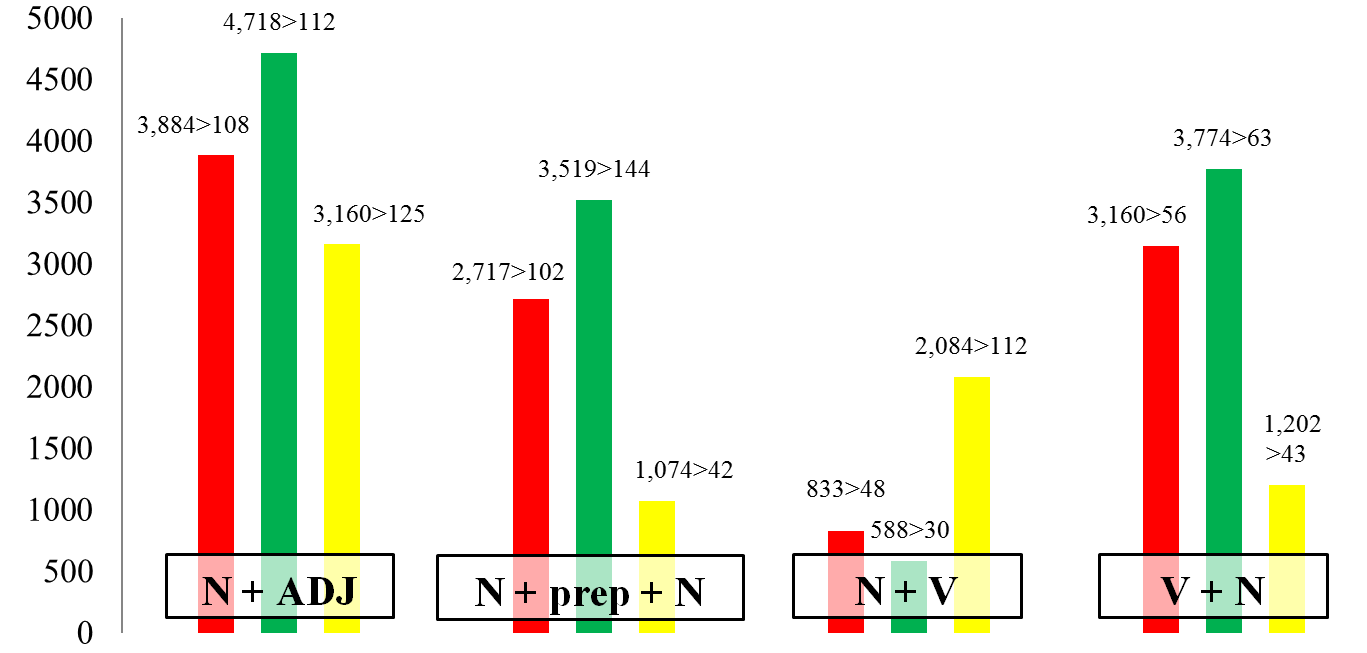
\includegraphics[width=1.0\textwidth]{./figures/1-3.png}
\definecolor{LSPdarkgreen}{RGB}{0,176,80}
\begin{tikzpicture}
\begin{axis}[set layers=axis on top,ybar, symbolic x coords={N + ADJ,N + prep + N,N + V,V + N}, xtick=data, nodes near coords, nodes near coords align={vertical}, every node near coord/.append style={rotate=90, anchor=west}, axis x line*=bottom, axis y line*=left, tickwidth=0pt, ymin=0, bar width=15, width=\textwidth, height={}, x tick label style={font=\bfseries, yshift=.75cm, draw, fill=gray!20, opacity=0.75}]
\addplot [fill=red, draw=none, point meta=explicit symbolic] coordinates {(N + ADJ,3884)[3884\textgreater 108] (N + prep + N,2717)[2717\textgreater 102] (N + V,833)[833\textgreater 48] (V + N,3160)[3160\textgreater 56]};
\addplot [fill=LSPdarkgreen, draw=none, point meta=explicit symbolic] coordinates {(N + ADJ,4718)[4718\textgreater 112] (N + prep + N,3519)[3519\textgreater 144] (N + V,588)[588\textgreater 30] (V + N,3774)[3774\textgreater 63]};
\addplot [fill=yellow, draw=none, point meta=explicit symbolic] coordinates {(N + ADJ,3160)[3160\textgreater 125] (N + prep + N,1074)[1074\textgreater 42] (N + V,2084)[2084\textgreater 112] (V + N,1202)[1202\textgreater 43]};

\end{axis}
\end{tikzpicture}
\caption{Lexical collocations (quantitative findings)} \label{fig:6:3}
\end{figure}

Overall, the analysis of \textsc{cospe} has revealed a balanced picture: CospIT contains the highest number of collocations with a nominal base, followed by CospES and CospIT. The only exception is the N + V pattern which shows a higher number of collocations in CospEN (2,084 vs. 112 types).

The most frequent lexical combination in the three subcorpora is N + \textsc{adj} (CospIT: 4,718, CospES: 3,884, CospEN: 3,160). However, the total number of types is higher in the English subcorpus (125) which seems to point to a higher lexical variation in English and Welsh criminal judgments. Also the V + N pattern, where the N functions as direct object of the sentence, displays a high number of collocations: 3,774 in CospIT, 3,160 in CospES and 1,202 in CospEN. Yet, a relatively lower number of types of collocations has emerged (CospES: 56, CospIT: 63, CospEN: 43) which could be interpreted as a higher level of repetition or lower lexical variation. Finally, the N + prep + N pattern shows a trend which is similar to N + \textsc{adj}: CospIT displays the highest number of collocations (3,519 vs. 144 types), followed by CospES (2,717 vs. 102) and CospEN (1,074 vs. 42).

A general trend can be outlined: the English subcorpus contains a lower frequency of lexical collocations, which is \enlargethispage{1\baselineskip} indeed an important quantitative result (see \sectref{sec:6:7}).

The quality analysis of these phraseological units revealed that lexical collocations play a key role in the genre under analysis and significantly contribute to the “taste” of judicial style which translators have to recreate in their target texts. The comparison with the reference corpora showed that such phraseological units are much more frequent in judicial language than in general language. This is also due to the presence of the judicial term as node of the collocations extracted (e.g. “appropriate sentence” 12.39 in CospEN vs. 0.12 in the \textsc{bnc}; “fairness of the trial” 15.4 in CospEN vs. 0.04 in the \textsc{bnc}; “allow* the appeal” 96.2 in CospEN vs. 1.07 in the \textsc{bnc}). For an in-depth analysis of the qualitative results, see \citep[241--252][]{Pontrandolfo2013a}.

\subsubsection{Routine formulae}
Routine formulae or phrases are “recurring lexical sequences, of different length, that develop in the case-law tradition and are usually collected in formularies” \citep[28--29]{Kjær1990}. The following examples have been extracted from \textsc{cospe}:

\begin{itemize}
\item \textbf{ES}: \textit{Así por esta nuestra Sentencia, lo pronunciamos, mandamos y firmamos; Que debo estimar y estimo; Leída y publicada ha sido la anterior sentencia por el Magistrado Ponente} […]
\item \textbf{IT}: \textit{Con la recidiva reiterate infraquinquennale; Indica in giorni X il termine per il deposito della sentenza};
\item \textbf{EN}: \textit{Judgment approved by the court for handing down; I would allow the appeal and quash the judgment; I have had the advantage of reading in draft the opinions of all my noble and learned friends}
\end{itemize}

These standardised formulae have been treated combining the insights provided by the genre analysis (Swales 1990, Bhatia 1993). In other terms, routine formulae have been clustered into the five main “moves” of criminal judgments: heading (EN), facts (H), legal background (D), operative part (F), final provisions (DIL). \figref{fig:6:4} shows the quantitative results.

\begin{figure}
% 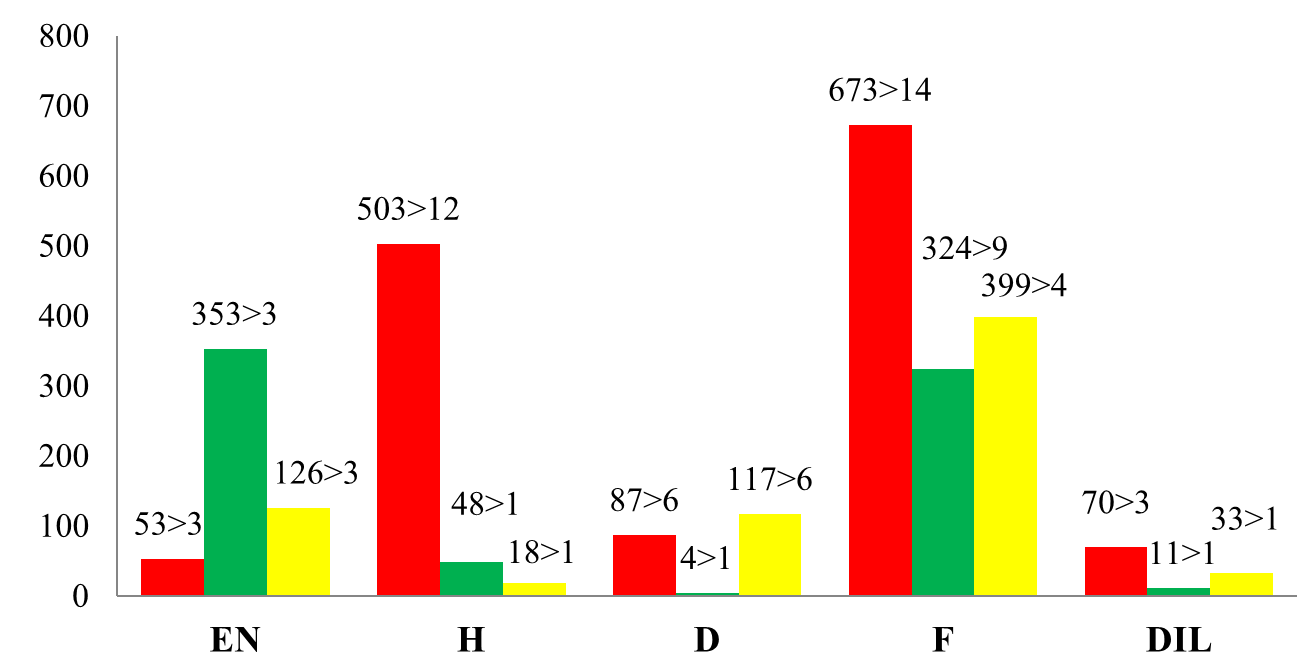
\includegraphics[width=1.0\textwidth]{./figures/1-4.png}
\definecolor{LSPdarkgreen}{RGB}{0,176,80}
\pgfplotsset{every axis/.append style={font=\normalfont}}
\begin{tikzpicture}
\begin{axis}[ybar, symbolic x coords={EN,H,D,F,DIL}, xtick=data, nodes near coords, nodes near coords align={vertical}, every node near coord/.append style={rotate=90, anchor=west}, axis x line*=bottom, axis y line*=left, tickwidth=0pt, ymin=0, bar width=15, width=\textwidth, height={}, x tick label style={font=\bfseries}]
\addplot [fill=red, draw=none, point meta=explicit symbolic] coordinates {(EN,53)[53\textgreater  3] (H,503)[503\textgreater  12] (D,87)[87\textgreater  6] (F,673)[673\textgreater  14] (DIL,70)[70\textgreater  3]};
\addplot [fill=LSPdarkgreen, draw=none, point meta=explicit symbolic] coordinates {(EN,353)[353\textgreater  3] (H,48)[48\textgreater  1] (D,4)[4\textgreater  1] (F,324)[324\textgreater  9] (DIL,11)[11\textgreater  1]};
\addplot [fill=yellow, draw=none, point meta=explicit symbolic] coordinates {(EN,126)[126\textgreater  3] (H,18)[18\textgreater  1] (D,117)[117\textgreater  6] (F,399)[399\textgreater  4] (DIL,33)[33\textgreater  1]};

\end{axis}
\end{tikzpicture}
\caption{Routine formulae (quantitative findings)} \label{fig:6:4}
\end{figure}

In general terms, the Spanish criminal judgments present the highest number of routine formulae (1,386), compared to the Italian (740) and English (693) ones. As far as the rhetorical sections (moves) are concerned, the most standardised section of the judgment is the operative part (decision) (CospES: 674, CospEN: 399, CospIT: 324), followed by the heading (CospIT: 353, CospEN: 126, CospES: 53). A high frequency of routine formulae is also found in the facts section of the Spanish judgments (503 instances distributed along 12 types), compared with the Italian (48 vs. 1) and English (18 vs. 1) ones. The legal sections (CospEN: 117, CospES: 87 and CospIT: 4) and the final provisions (CospES: 70. CospEN: 33 and CospIT: 11) are the moves which display the lower number of standardised sequences.

The quality analysis of these phraseological patterns \citep[255--261]{
Pontrandolfo2013b} confirmed that the genre under examination contains a high degree of standardisation and homogeneity, although these two traits do not seem to characterise the English and Welsh judgments. As far as the comparison with the general language is concerned, routine formulae are hardly present in reference corpora.

The following final section attempts to interpret these results in the light of the two different legal traditions characterising the three systems: common law on the one hand (England and Wales), and civil law on the other hand (Spain and Italy).

\section{Discussion} \label{sec:6:7}
Results thus obtained have confirmed the three initial hypotheses.

As far as the first research question is concerned, criminal judgments display a high percentage of phraseological units in the three subcorpora. The comparison between frequency of co-occurrence of the extracted phraseologisms and their frequency in reference corpora (e.g. \textsc{crea} for Spanish, \textsc{coris}/\textsc{codis} for Italian and \textsc{bnc} for English) confirms that phraseology is indeed a key lexico-syntatic feature of this genre and it is part of judges’ idiosyncratic drafting conventions.
 
As far as the second research question is concerned, the English subcorpus shows a lower degree of standardisation and, consequently, a lower percentage of phraseological units, compared to the Spanish and the Italian subcorpora. As illustrated extensively elsewhere (see, in particular, \citealt{Pontrandolfo2013a}: 144--145), although criminal judgments have the same function in the three judicial systems, their content and their textual realisation differ significantly. English and Welsh judgments are the results of a long oral tradition. Common-law judges have their personal style, that they use to justify their decisions in a personal, subjective way. There are no constrictions in the outline or content of the texts they produce, also because, unlike the other two, the English and Welsh judicial system lacks important reference texts, such as the Spanish or Italian Codes of Criminal Procedure. This affects the standardisation and the different phraseological weight between English and Welsh judgments on the one hand, and Spanish and Italian on the other.

As far as the third research question is concerned, the results of the analysis interestingly highlight the comparability of phraseologims found in the Spanish, Italian and English criminal judgments. The presence of “parallel phraseologims” is of crucial importance in terms of legal translation. Functional equivalence \citep[see][]{TogniniBonelli1996} can be achieved in most cases, as can be demonstrated by applying the “translation by collocation” approach \citep[see][]{TogniniBonelli2004,Pontrandolfo2013a}. From the perspective of judicial reasoning, the results seem to point to the existence of a “legal/judicial grammar”, especially in the case of Spain and Italy, namely a series of phraseological, idiosyncratic conventions that typically recur in judicial discourse.

\section{Conclusions}
As far as the applications of the present study are concerned, the specialised phraseologisms yielded by the research can serve, first and foremost, phraseographic purposes, providing legal translators with a practical guide containing useful information on the contexts of use and, above all, the frequency of some expressions \citep[see][]{Lombardi2004}. Such tool will help translators in the stylistic rendering of their target texts and “reassure” them about the appropriate linguistic and legal use of specialised  phraseological combinations.

The extracted phraseological units can also be used for lexicographic purposes, integrating already existing legal databases or dictionaries, or constituting the basis for new phraseological resources specifically designed for legal language.

However, the most valuable application of the study is in the training of legal translators. Familiarising with the “routines” of the genre \citep{Hatim1997}, as well as mastering their use (both at receptive and productive level) are crucial factors in legal translators’ training \citep[see][]{Garzone2007}. Phraseology is also a fundamental way for trainees to understand the conceptual relation between the different elements of a specialised text. While terms map out the legal system and therefore pertain to the knowledge (discipline) space in each judicial system, phraseology structures the texts of the legal domain. Getting familiar with the specific phraseology of the register of a discourse community will therefore bring about not only a better knowledge of the genre, but also an enhanced competence in the process of writing and reading specialised registers \citep[see][]{Williams2002}. A tool like \textsc{cospe} can help legal translators improve their phraseological competence, showing them how to produce texts that fit the stylistic conventions of the target language original texts.

One of the future challenges will be that of enlarging \textsc{cospe} to include other legal genres, as well as a parallel corpus. This would allow a replication of the study with different legal texts, focusing on a comparison between phraseological behaviours across different genres. Furthermore, a new hypothesis will be tested:\footnote{Future studies will attempt to answer the following research question: What is the relationship between phraseology and the quality of the target text? In other words, is there a relationship between the translators’ phraseological competence and the final quality of the text? Can phraseology contribute to improving the quality of translated texts, and if so, how?} phraseology as a quality-enhancing factor in legal translation.

 \todo{I removed the `Bibliography' heading here as one is already created by \textbackslash printbibliography}

%\section{Bibliography}


\printbibliography[heading=subbibliography,notkeyword=this]

\end{document}